\documentclass[a4paper, 14pt]{extarticle}
\usepackage{enumitem}
\usepackage{fefutitle}
\usepackage{xcolor}
\usepackage{amsmath}
\usepackage{graphicx}
\usepackage[justification=centering]{caption}
\usepackage{float}

\begin{document}
	\fefutitle{6}
	\pagebreak	

	\section{Определение цели}
		Вода -- основной элемент в жизни организма и Земля покрыта ей на $71\%$. Движение воды -- течения. Течения могут иметь различные частица с различными температурами. В данной лабораторной работе необходимо создать модель водоема с течением и и частицами, которые обладают собственными температурами.
		
	\section{Создание математической модели}
		Все частицы примем за материальную точку. Создадим их $n$  штук со случайными координатами $x_i, y_i$  от 0 до 1.
		И каждой частице присвоим свою концентрацию:
		\[ C_i = \begin{cases} -1, \ \text{если} \ y_i < 0.5 \\ \phantom{-} 1, \ \text{если} \ y_i \geq 0.5 \end{cases}\]
		
		Траекторию движения частиц будет описывать следующая функция:
		\[ \psi = \sin(2\pi x) \cdot \sin(\pi y) \]
		
		Скорость частиц по осям OX и OY:
		\[ \begin{cases}
				\dfrac{dx_i}{dt} = u(x_i, y_i) = -\dfrac{\partial \psi}{\partial x} = -2\pi \cos(2\pi x_i) \cdot \sin(\pi y_i), \\
				\dfrac{dy_i}{dt} =\upsilon (x_i, y_i) = \phantom{-}\dfrac{\partial \psi}{\partial y} = \phantom{-} \pi \sin(2\pi x_i) \cdot \cos(\pi y_i)
			\end{cases}
		\]

	\section{Реализация модели}
		Модель была реализована в Python.
		\begin{figure}[H]
			\begin{minipage}{0.5\textwidth}
				\centering
				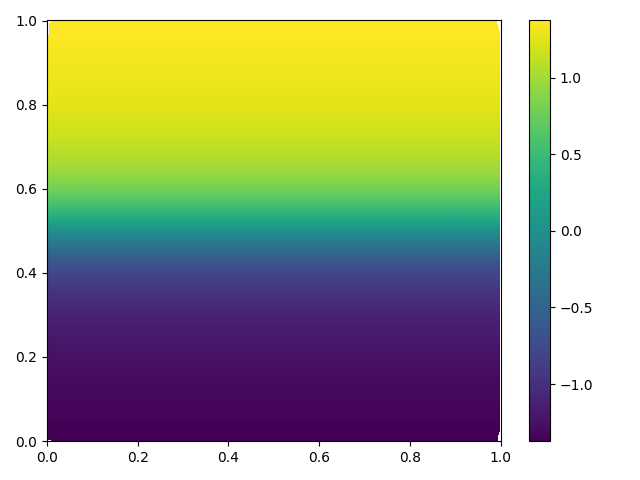
\includegraphics[width = \linewidth]{1.png}
			\end{minipage}\hfill
			\begin{minipage}{0.5\textwidth}
				\centering
				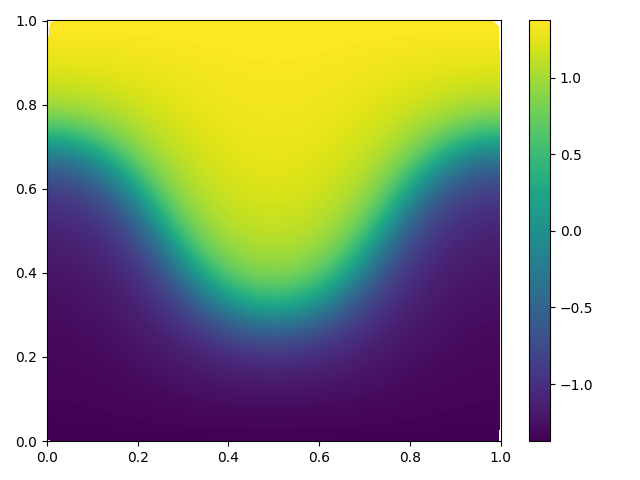
\includegraphics[width = \linewidth]{2.png}
			\end{minipage}\hfill
		\end{figure}
	
		\begin{figure}[H]
			\begin{minipage}{0.5\textwidth}
				\centering
				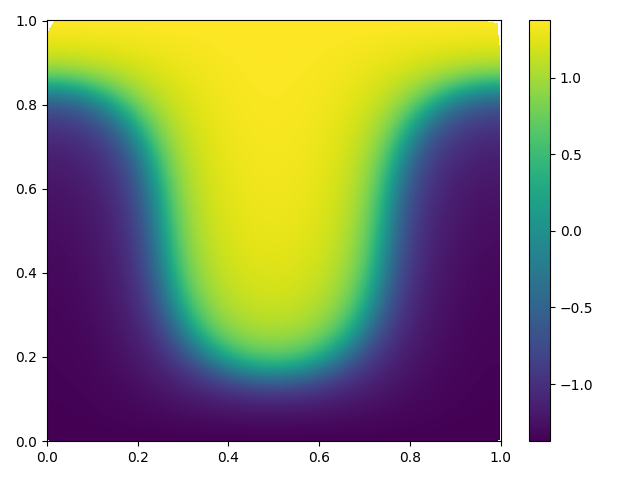
\includegraphics[width = \linewidth]{3.png}
			\end{minipage}\hfill
			\begin{minipage}{0.5\textwidth}
				\centering
				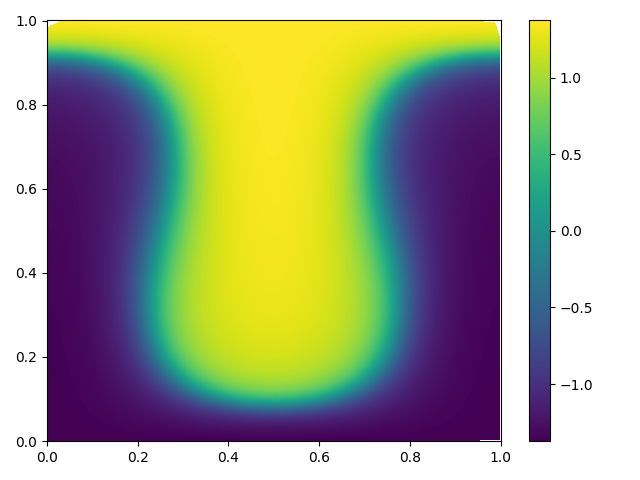
\includegraphics[width = \linewidth]{4.png}
			\end{minipage}\hfill
		\end{figure}
	
		\begin{figure}[H]
			\begin{minipage}{0.5\textwidth}
				\centering
				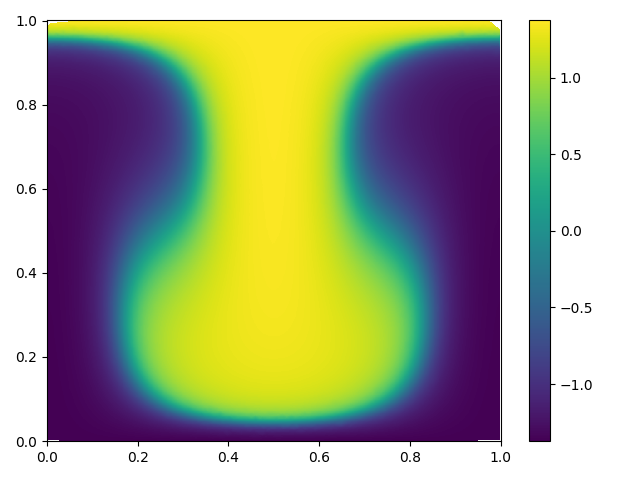
\includegraphics[width = \linewidth]{5.png}
			\end{minipage}\hfill
			\begin{minipage}{0.5\textwidth}
				\centering
				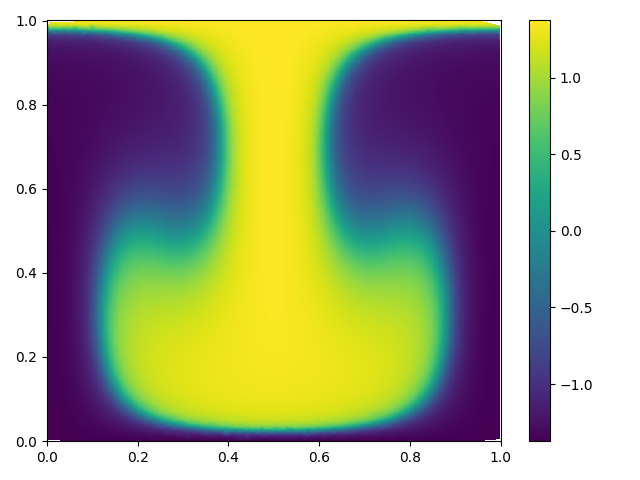
\includegraphics[width = \linewidth]{6.png}
			\end{minipage}\hfill
		\end{figure}
	
		\begin{figure}[H]
			\begin{minipage}{0.5\textwidth}
				\centering
				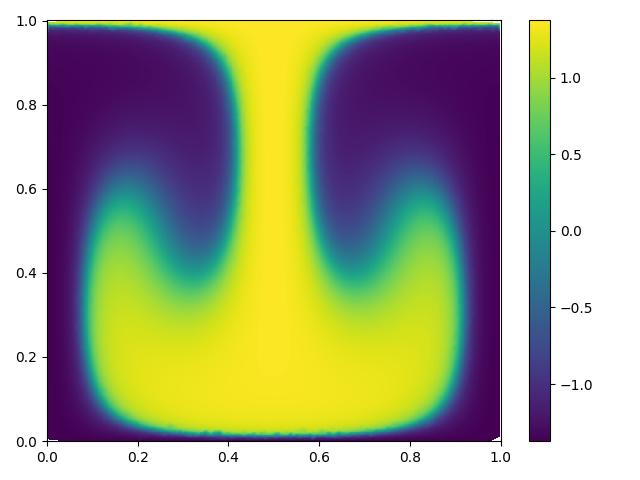
\includegraphics[width = \linewidth]{7.png}
			\end{minipage}\hfill
			\begin{minipage}{0.5\textwidth}
				\centering
				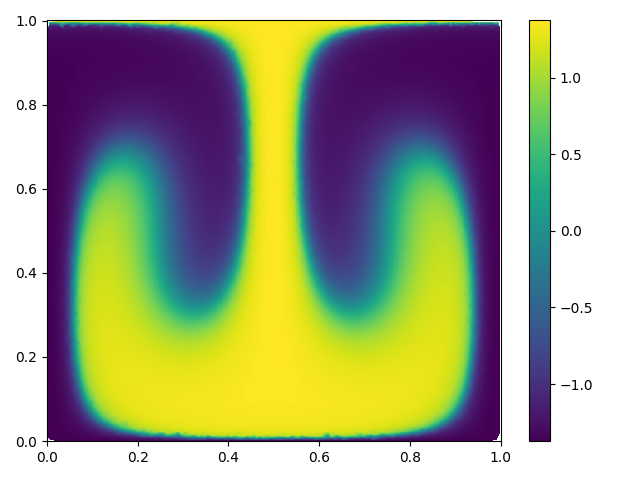
\includegraphics[width = \linewidth]{8.png}
			\end{minipage}\hfill
		\end{figure}
	
		\begin{figure}[H]
			\begin{minipage}{0.5\textwidth}
				\centering
				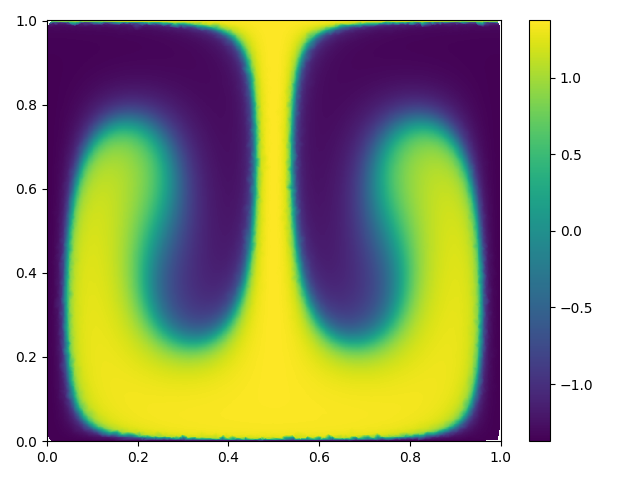
\includegraphics[width = \linewidth]{9.png}
			\end{minipage}\hfill
			\begin{minipage}{0.5\textwidth}
				\centering
				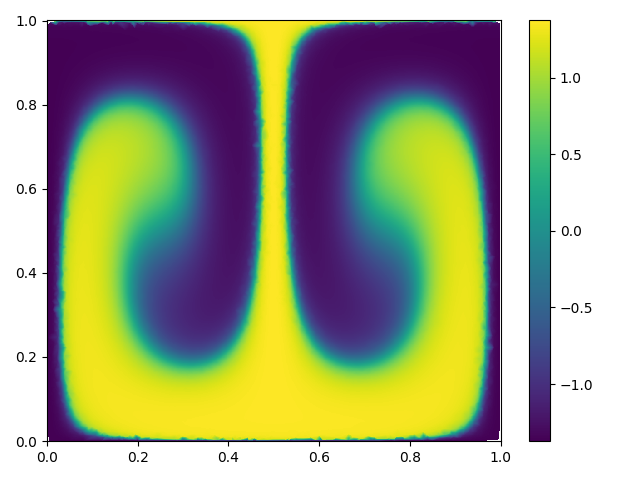
\includegraphics[width = \linewidth]{10.png}
			\end{minipage}\hfill
		\end{figure}
		
	\section{Вывод}
		
\end{document}	